\documentclass[conference, a4paper]{IEEEtran}
\IEEEoverridecommandlockouts

\usepackage{cite}
\usepackage{amsmath,amssymb,amsfonts}
\usepackage{algorithmic}
\usepackage{graphicx}
\usepackage{textcomp}
\usepackage{xcolor}
\usepackage{float}
\usepackage{caption}
\usepackage{subcaption}

\graphicspath{{../../graphics/rectangular_dielectric_waveguide}{../../graphics/comsol_individual_waveguide}}

\def\BibTeX{{\rm B\kern-.05em{\sc i\kern-.025em b}\kern-.08em
    T\kern-.1667em\lower.7ex\hbox{E}\kern-.125emX}}
\begin{document}

\title{Coupled Mode Theory and 50/50 Splitter}

\author{\IEEEauthorblockN{Eduardo A. V. Souza, RA: 250950}
\IEEEauthorblockA{\textit{"Gleb Wataghin" Institute of Physics} \\
\textit{UNICAMP}\\
Campinas, Brazil}
\and
\IEEEauthorblockN{Ivan Prearo (RA 237215)}
\IEEEauthorblockA{\textit{"Gleb Wataghin" Institute of Physics} \\
\textit{UNICAMP}\\
Campinas, Brazil}}

\maketitle

\begin{abstract}
    hgjg
\end{abstract}

\begin{IEEEkeywords}
    Waveguides, Coupled Mode Theory, Beamsplittersnsing.
\end{IEEEkeywords}

\section{Introduction}
\label{sec:intro}

\section{Infinite dielectric waveguide}
\label{sec:slab}

\subsection{Theory development}
\label{subsec:slab_theory}

\subsection{Numerical analysis}
\label{subsec:slab_num}

\section{Rectangular dielectric waveguide}
\label{subsec:rectangle}

\subsection{Theoretical development}
\label{subsec:rectangle_theory}

\subsection{Solo waveguide}
\label{subsec:rectangle_solo}

\begin{figure}[H]
    \centering
    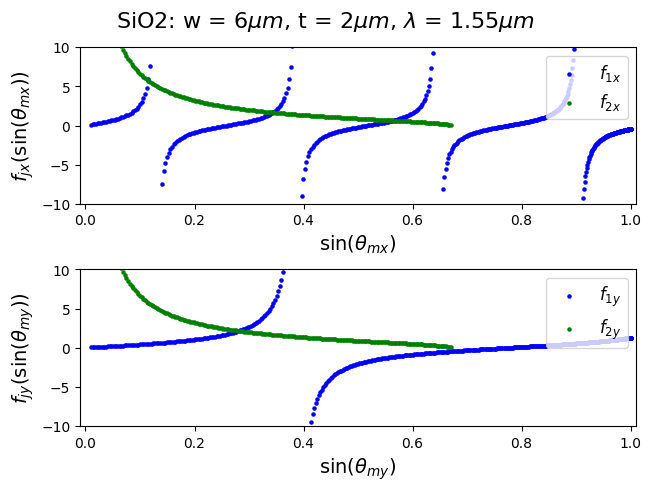
\includegraphics[scale=0.5]{characteristic_equation_SiO2.png}
    \caption{}
    \label{fig:cha_eq}
\end{figure}

\begin{figure}[H]
    \centering
    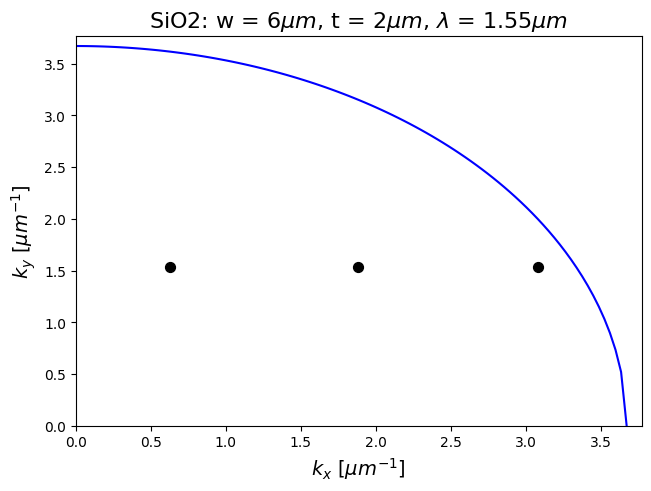
\includegraphics[scale=0.5]{modeshell_SiO2.png}
    \caption{}
    \label{fig:mode_shell}
\end{figure}

\begin{figure}[H]
    \centering
    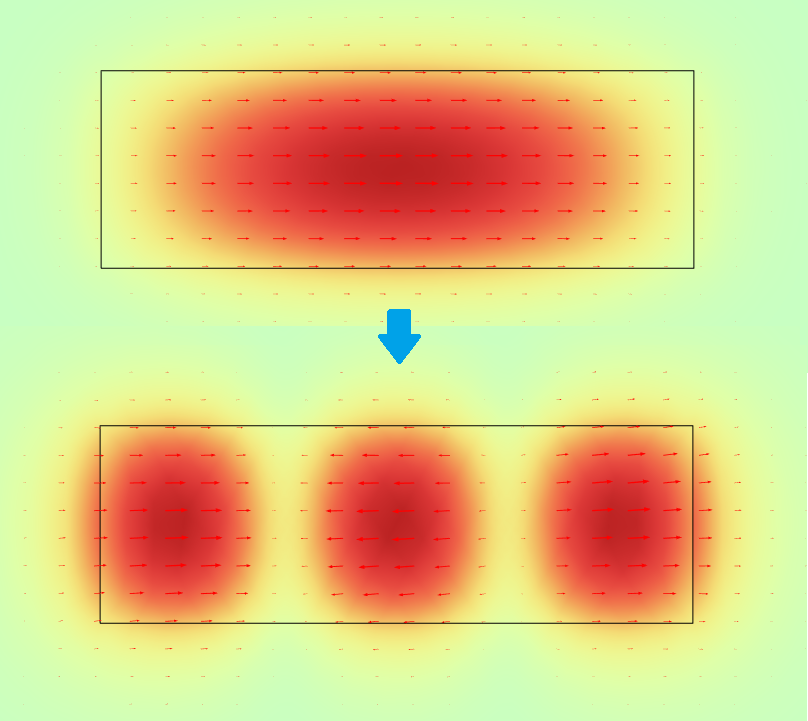
\includegraphics[scale=0.3]{normE_different_modes.png}
    \caption{}
    \label{fig:dif_modes}
\end{figure}

\subsection{Coupled waveguide}
\label{subsec:rectangle_coupled}

\section{Conclusion}
\label{sec:conclusion}

\section*{Appendix}
\label{sec:appendix}

% \bibliographystyle{IEEEtran}
% \bibliography{References}


\end{document}
